% Autor: Leonhard Segger, Alexander Neuwirth
% Datum: 2017-10-30
\documentclass[
	% Papierformat
	a4paper,
	% Schriftgröße (beliebige Größen mit „fontsize=Xpt“)
	12pt,
	% Schreibt die Papiergröße korrekt ins Ausgabedokument
	pagesize,
	% Sprache für z.B. Babel
	ngerman
]{scrartcl}

% Achtung: Die Reihenfolge der Pakete kann (leider) wichtig sein!
% Insbesondere sollten (so wie hier) babel, fontenc und inputenc (in dieser
% Reihenfolge) als Erstes und hyperref und cleveref (Reihenfolge auch hier
% beachten) als Letztes geladen werden!

\usepackage{tikz}
\usetikzlibrary{calc,patterns,angles,quotes} % loads some tikz extensions\usepackage{tikz}
\usetikzlibrary{babel}

% Silbentrennung etc.; Sprache wird durch Option bei \documentclass festgelegt
\usepackage{babel}
% Verwendung der Zeichentabelle T1 (Sonderzeichen etc.)
\usepackage[T1]{fontenc}
% Legt die Zeichenkodierung der Eingabedatei fest, z.B. UTF-8
\usepackage[utf8]{inputenc}
% Schriftart
\usepackage{lmodern}
% Zusätzliche Sonderzeichen
\usepackage{textcomp}

% Mathepaket (intlimits: Grenzen über/unter Integralzeichen)
\usepackage[intlimits]{amsmath}
% Ermöglicht die Nutzung von \SI{Zahl}{Einheit} u.a.
\usepackage{amssymb}
% mehr symbole plox
\usepackage{siunitx}
% Zum flexiblen Einbinden von Grafiken (\includegraphics)
\usepackage{graphicx}
% Abbildungen im Fließtext
\usepackage{wrapfig}
% Abbildungen nebeneinander (subfigure, subtable)
\usepackage{subcaption}
% Funktionen für Anführungszeichen
\usepackage{csquotes}
\MakeOuterQuote{"}
% Zitieren, Bibliografie
\usepackage[sorting=none]{biblatex}


% Zur Darstellung von Webadressen
\usepackage{url}
%chemische Formeln
\usepackage[version=4]{mhchem}
% siunitx: Deutsche Ausgabe, Messfehler getrennt mit ± ausgeben
\usepackage{floatrow}
\floatsetup[table]{capposition=top}
\usepackage{float}
% Verlinkt Textstellen im PDF-Dokument
\usepackage[unicode]{hyperref}
% "Schlaue" Referenzen (nach hyperref laden!)
\usepackage{cleveref}
\sisetup{
	locale=DE,
	separate-uncertainty
}
\bibliography{References}

\begin{document}

	\begin{titlepage}
		\centering
		{\scshape\LARGE Versuchsbericht zu \par}
		\vspace{1cm}
		{\scshape\huge Optische Fouriertransformation \par}
		\vspace{2.5cm}
		{\LARGE Gruppe BA-C-04 \par}
		\vspace{0.5cm}

		{\large Alexander Neuwirth (E-Mail: a\_neuw01@wwu.de) \par}
		{\large Leonhard Segger (E-Mail: l\_segg03@uni-muenster.de) \par}
		\vfill

		durchgeführt am 17.06.2019\par
		betreut von\par
		{\large Florian Schepers}

		\vfill

		{\large \today\par}
	\end{titlepage}
	\tableofcontents
	\newpage


	\section{Kurzfassung}
	% Hypothese	und deren Ergebnis, wenn Hypothese ist, dass nur Theorie erfüllt, sagen: Erwartung: Theorie aus einführung (mit reflink) erfüllt
	% Ergebnisse, auch Zahlen, mindestens wenn's halbwegs Sinn ergibt
	% Was wurde gemacht
	% manche leute wollen Passiv oder "man", manche nicht
	In diesem Versuch werden verschiedene Aufbauten verwendet, um die Eingenschaften der optischen Fouriertransformation zu zeigen.
	Zunächst wird gezeigt, dass die Franuhofer-Beugung im Fernfeld zu eienr Fouriertransformation des Objekts führt, während dies im Nahfeld nicht der Fall ist, indem das Beugungsbild eines Gitters bei verschiedenen Schirmabständen aufgenommen wird.
	Dann werden für fünf verschiedene Gitter die Gitterabstände aus den Abständen der Beugungsordnungen auf dem Schirm bestimmt.


  \section{Theorie}
	% wdh. Texte
	% wdh. Besprechung


	\subsection{Kohärenz} %TODO hier nötig? Theoretisch genauso sehr wie beim letzten.
	Der signifikante Unterschied zwischen einem Laser und einer Glimmlampe besteht in der Fähigkeit zur Interferenz.
	Die Lichtwellen, die den Laser verlassen haben eine feste Phasenbeziehung, weshalb nach Trennung des Strahls Interferenz zwischen beiden Teilstrahlen zu beobachten ist.

	Bei der qualitativen Beschreibung der Interferenzfähigkeit unterscheidet man zwischen räumlicher und zeitlicher Kohärenz.
	Zeitliche Kohärenz kann über Autokorrelation mittels des Michelson-Interferometers gemessen werden.
	Die Kohärenzlänge ist definiert durch den Abstand (optische Wegdifferenz), der die Länge eines Arms des Interferometers vom Interferenzmaximum wegbewegt werden kann, bevor die durch die Interferenz erzeugte Autokorrelationsfunktion nicht mehr über $1/\text{e}$ steigt.
	Die Kohärenzlänge ergibt sich aus der Monochromatizität des Lichts, da sich bei perfekt monochromatischem Licht die Phasenbeziehung über keine Entfernung ändert.
	Die räumliche Kohärenz kann mittels eines Doppelspaltexperiments (oder des Young-Interferometers) gemessen werden, da sie die Phasenbeziehung innerhalb einer Wellenfront beschreibt und der Doppelspalt Interferenz zwischen unterschiedlichen Teilen der Wellenfront realisiert.
	%TODO copy paste sinn checken

	\subsection{Fouriertransformation}
	Die Fouriertransformation erlaubt die Zerlegung eines Signals in seine Teilfrequenzen.
	Sie basiert auf der Fourierreihe, erlaubt aber auch die Transformation zeitlich begrenzter Signale.
	Sie kann auf zweidimensionale Bilder übertragen werden, die dann in räumliche Frequenzen in x- und y-Richtung zerlegt werden.
	Die räumliche Transformation erfolgt dann gemäß
	\begin{equation}
		\mathcal{F}[f(x,y)](\nu_x, \nu_y) = \int _{-\infty}^{\infty} \int^{\infty}_{-\infty} f(x,y) \exp (-2\pi i (\nu_x x + \nu_y y)) \mathrm{d} x \mathrm{d} y = F (\nu_x , \nu_y)
	\end{equation}
	und die Rücktransformation gemäß
	\begin{equation}
		\mathcal{F}^{-1}[F (\nu_x , \nu_y))](x, y) = \int _{-\infty}^{\infty} \int^{\infty}_{-\infty} F(\nu_x , \nu_y) \exp (2\pi i (\nu_x x + \nu_y )) \mathrm{d} \nu_x \mathrm{d} \nu_y = f (x , y)
	\end{equation}
	(vgl. \cite{Anleitung}).

	Räumliche Frequenzen tauchen im Beugungsbild als Punkte auf.

	\subsection{Fraunhofer-Beugung}
	\label{sec_fraunhofer}

	Was die Fraunhofer-Beugung angeht, reicht es, sich hier darauf zu beschränken, dass durch die Beugung an Spalten und Gittern im Fernfeld eine Fouriertransformation des Spalts bzw. Gitters auftritt.
	Durch eine Linse kann diese Fouriertransformation rückgängig gemacht werden und das Bild ins Nahfeld geholt werden.
	Dabei findet eine Spiegelung und Skalierung des Bildes statt.

	Im Nahfeld wird die Beugung demhingegen durch die Fresnel-Beugung beschrieben.

	\begin{figure}[H]
			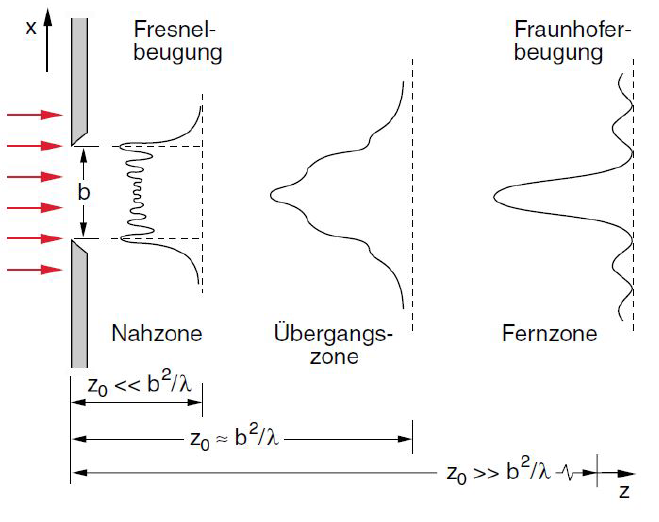
\includegraphics[width=1\linewidth]{img/fraunfresnel}
			\caption{
				Fresnel- und Fraunhoferbereiche relativ zum Abstand der beugenden Struktur. \cite{Anleitung}
			}
			\label{fig_fraunfresnel}
	\end{figure}

	\subsection{Beugung am Gitter}
	\label{sec_gitterbeug}

	Einzelspalte entsprechen Rechteckfunktionen, die transformiert Funktionen der Form $\sin{x}/x$ ergeben.
	Bei einem Doppelspalt tauchen zusätzlich Nebenmaxima auf und bei Gittern ergeben sich einzelne Hauptmaxima hoher Intensität.

	Die Beugung am Gitter ergibt gemäß \cite{Anleitung} bei Spaltabstand $b$, Spaltzahl $N$ und Abstand $d$ die Intensitätsverteilung:
	\begin{equation}
		I(\theta) = I_0 \cdot \text{sinc}^2\left(\frac{N \pi d \sin \theta}{\lambda} \right) \cdot \text{sinc}^2\left(\frac{\pi b \sin \theta}{\lambda} \right)
	\end{equation}


	Für das $k$-te Maximum gilt dann:
	\begin{equation}
		b \cdot \sin{\theta} = k \lambda
	\end{equation}
	Für kleines $\theta$ gilt $\theta \approx \sin{\theta} \approx \tan{\theta}=\frac{u}{d}$, wobei $u$ der Abstand eines Maximas der Ordnung $k$ zur nullten Ordnung ist und somit:
	\begin{equation}
		\label{eq_beug}
		b = \frac{k\lambda d}{u}
	\end{equation}
	$d$ ist dabei der Abstand zwischen Gitter und Schirm.

	\subsection{4-f-Aufbau}
	Um eine Filterung einzelner Frequenzen aus einer optischen Fouriertransformation zu erlauben, kann der sog. 4-f-Aufbau verwendet werden.
	Dazu werden wie in \cref{fig_4f_schema} dargestellt zwei Linsen verwendet, die jeweils im Abstand ihrer Brennweite zwischen Objektebene und Fourierebene bzw. Fourierebene und Bildebene stehen.
	Nun können mit Spalten eindimensionale Tiefpassfilter, mit Nadeln eindimensionale Hochpässe, mit Klarsichtfolien mit schwarzem Punkt zweidimensionale Hochpassfilter und mit Lochblenden zweidimensionale Tiefpässe realisiert werden.
	Diese erlauben es periodische Strukturen aus dem Bild zu entfernen.

	\begin{figure}[H]
			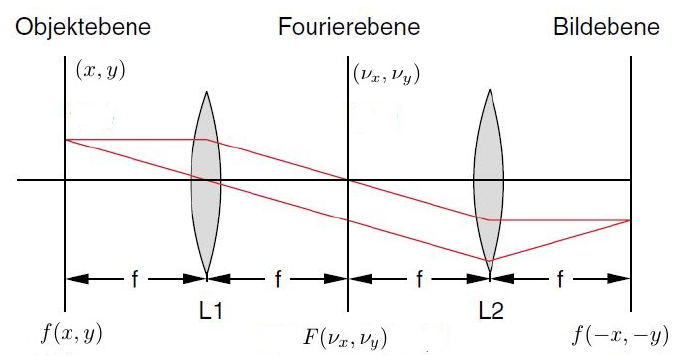
\includegraphics[width=1\linewidth]{img/4f_schema}
			\caption{
				Objekt-, Fourier- und Brennebene in einem 4-f-Aufbau aus zwei Linsen mit gleicher Brennweite. \cite{Anleitung}
			}
			\label{fig_4f_schema}
	\end{figure}

	\subsection{Dunkelfeldmethode}

	Durch Verwendung eines 4-f-Aufbaus mit einem Hochpassfilter lassen sich Phasenveränderungen durch das Objekt als Intensität auf dem Schirm sichtbar machen.
	Solche Phasenveränderungen können zum Beispiel durch heiße Luftströmungen auftreten, die einen leicht anderen Brechungsindex und somit eine andere Lichtgeschwindigkeit im Innern besitzen, als die umgebende Luft.

	\section{Grundaufbau}
	Es wird ein Helium-Neon-Laser auf einer \SI{4}{m} langen optischen Bank montiert.
	Am anderen Ende der Bank wird ein halbtransparenter Schirm aufgestellt, auf den von Hinten eine Digitalkamera gerichtet und fokussiert wird. %TODO "halbtransparent"?
	Der Laser wird mithilfe einer Lochblende parallel zur optischen Bank ausgerichtet.
	Wenn im Folgenden Linsen eingesetzt werden, wird mithilfe einer Markierung auf einem Schirm sichergestellt, dass der Laserstrahl nach Durchgang durch die Linse noch immer im Mittel parallel zur optischen Bank verläuft, der Laser also mittig durch die Linse läuft. %TODO im Mittel, weil ja nicht jeder Teilstrahl parallel ist. theoretisch auch im vorigen Satz
	Es wird die Länge in Pixeln eines Abstandes von \SI{10}{cm} anhand eines Lineals auf dem Schirm anhand der Digitalaufnahme gemessen, um den Umrechnungsfaktor von Pixeln in Abstand auf dem Schirm zu bestimmen.
	%TODO kp, ob du den Umrechnungsfaktor irgendwo hinpacken willst. und wo.
	Im Folgenden wird die Belichtungszeit der Kamera für jede Aufnahme individuell eingestellt, um eine optimale Abzählung der Peaks zu ermöglichen.
	Hierfür wird auch eine Überbelichtung in Kauf genommen.
	Dies verhindert einen Vergleich der Intensitäten zwischen einzelnen Aufnahmen, aber ein solcher ist auch nicht notwendig.

	\begin{figure}[H]
			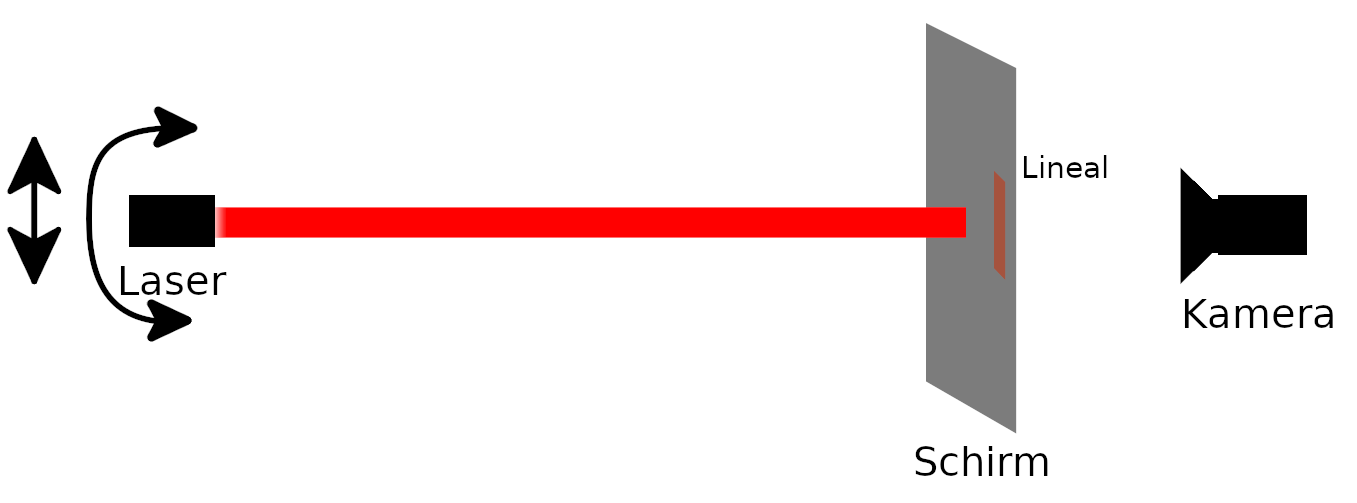
\includegraphics[width=1\linewidth]{img/grundaufbau}
			\caption{
				Der Grundaufbau. Der Laser wird parallel zur optischen Bank ausgerichtet.
			}
			\label{fig_grundaufbau}
	\end{figure}

	\section{Ergebnisse und Diskussion}
	%TODO ist das fine, dass ich das alles * gemacht habe?

	%\subsection{Unsicherheiten}
	%TODO Unsicherheiten
	\subsection{Unsicherheiten und Kalibration}
	Alle Unsicherheiten werden nach GUM bestimmt und berechnet.
	Für diese Berechnungen wurde die Python Bibliothek \enquote{uncertainties} herangezogen, welche den Richtlinien des GUM folgt.

	In \cref{fig_kalibration} ist ein exemplarisches Bild der Kamera mit sichtbarem Lineal abgebildet.
	Es ergibt sich ein Umrechnungsfaktor $\gamma$ von
	\begin{equation}
			\label{eq_kali}
			\gamma = \frac{\SI{10.0+-0.03}{cm}}{\SI{934+-0.3}{px}}=\SI{0.01071+-0.00003}{cm/px}.
	\end{equation}
	Wobei sich die Unsicherheit beim Ablesen des Lineals mit $u(l)=\frac{\SI{1}{mm}}{2\sqrt{6}}$ (analog, Dreiecksverteilung).
	Analog ergibt sich für die Pixelzahl $u(p)=\frac{\SI{1}{px}}{2\sqrt{6}}$.
	In \cref{eq_kali} wurden die Unsicherheiten zusätzlich mit $\sqrt{2}$ multipliziert, da um die Abstand zweier Punkte zumessen zweimal gemessen werden muss und sich die Fehler gemäß $\sqrt{u_1^2+u_2^2}$ fortpflanzen.

	Es wird sich im folgenden jedoch zeigen, dass die Unsicherheiten die dadurch entstehen, dass beispielweise Maxima nicht genau auf dem Schirm ablesbar sind, deutlich gegen über den der Kalibration überwiegen. %TODO verständlich?


	\begin{figure}[H]
		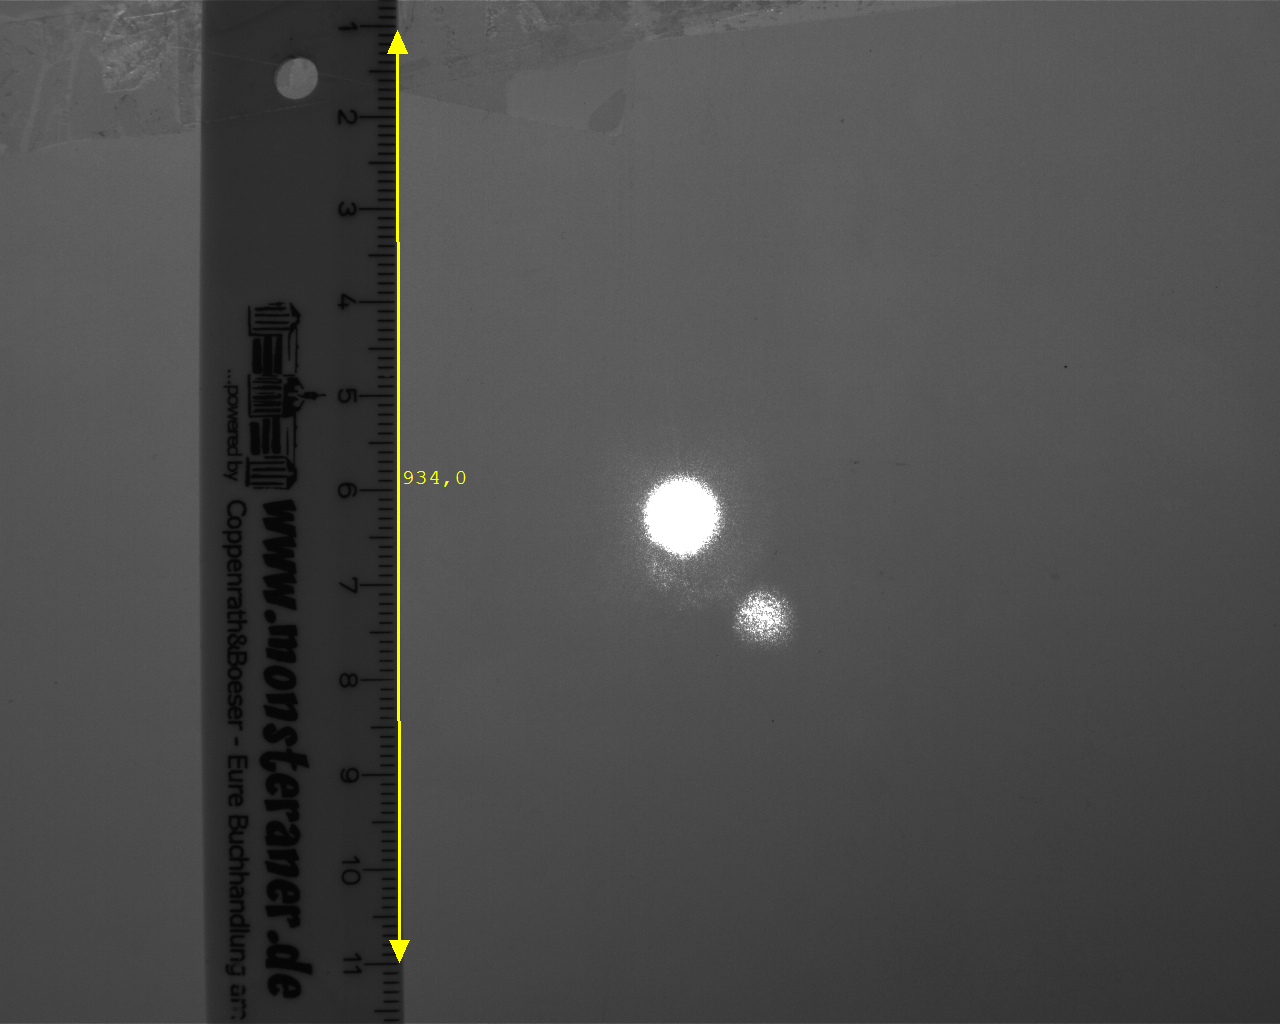
\includegraphics[width=0.7\linewidth]{raw/0/0_kalibration.png}
					\caption{
						Kalibration zur Umrechnung von Pixeln in Abstände.
						Der zweite kleinere Laserpunkt entsteht durch eine Ablenkung durch einen Graufilter vor dem Laser.
						Für die nachfolgenden Messungen wurde der Graufilter entfernt.
					}
					\label{fig_kalibration}
			\end{figure}


	\subsection{Übergang von Nah- zu Fernfeld}

	\subsubsection*{Methode}
	In den Strahlengang werden zwei Linsen mit $f_1=\SI{50}{mm}$ und $f_2=\SI{100}{mm}$ in einem Abstand von \SI{170}{mm} gebracht, um den Strahl zu kollimieren.
  Dann wird ein Gitter (später Gitter Nr.2) in den Strahl gebracht und in verschiedenen Abständen das Bild auf dem Schirm aufgenommen.

		\begin{figure}[H] %TODO Abstand d kann ich in alles ändern.
			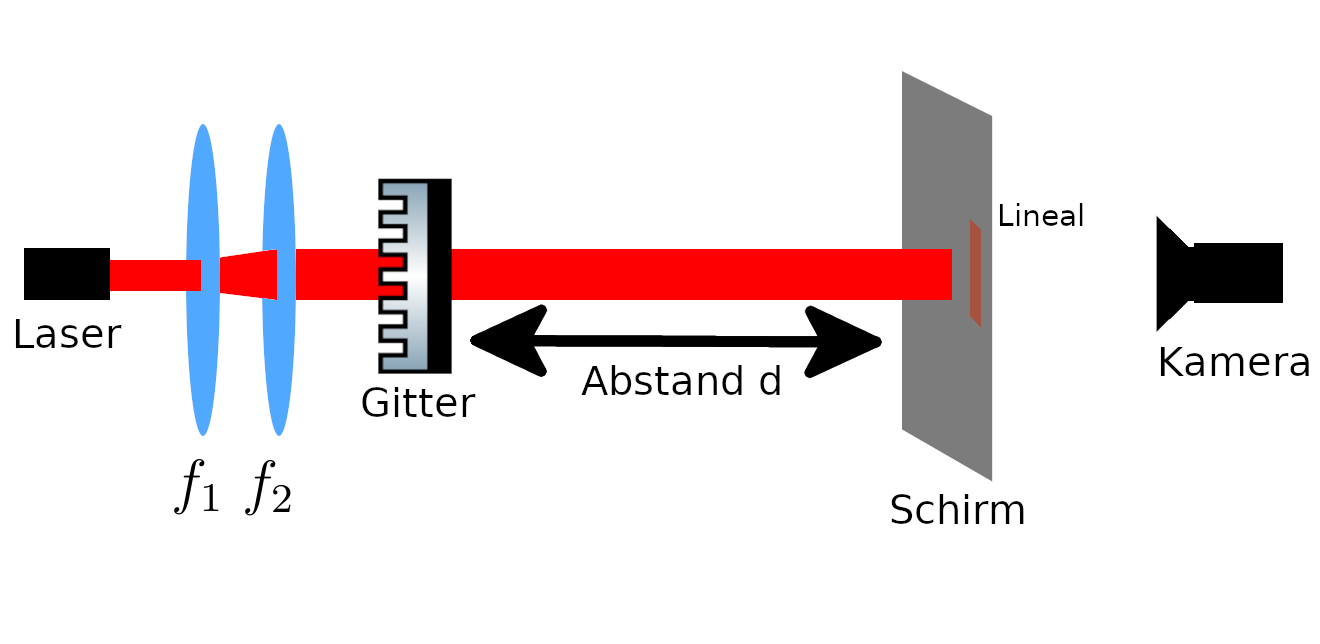
\includegraphics[width=1\linewidth]{img/nahfern}
					\caption{
						Aufbau zum Vergleich von Nah- und Fernfeld. Der Abstand zwischen den Kollimierungslinsen beträgt \SI{170}{mm}
					}
					\label{fig_nahfern}
			\end{figure}


	\subsubsection*{Beobachtung und Datenanalyse}
	% Allgemeine Beobachtungen
	% Einflüsse von veränderten Parametern auf Messung
	In \cref{fig_1_mix_1} sind sowohl aufgenommen Kamerabilder als auch logarithmische Intensitätsprofile abgebildet.
	Die Profile wurden hierbei aus einer anderen Aufnahme mit geringer Belichtungszeit gezogen, da hier eine Überbelichtung und somit ein Abschneiden der Peaks unerwünscht ist, während die Fotografien selbst mit höherer Belichtungszeit besser zu erkennen sind.

	\begin{figure}[H]
        \centering
        \begin{subfigure}[b]{0.4\textwidth}
            \centering
            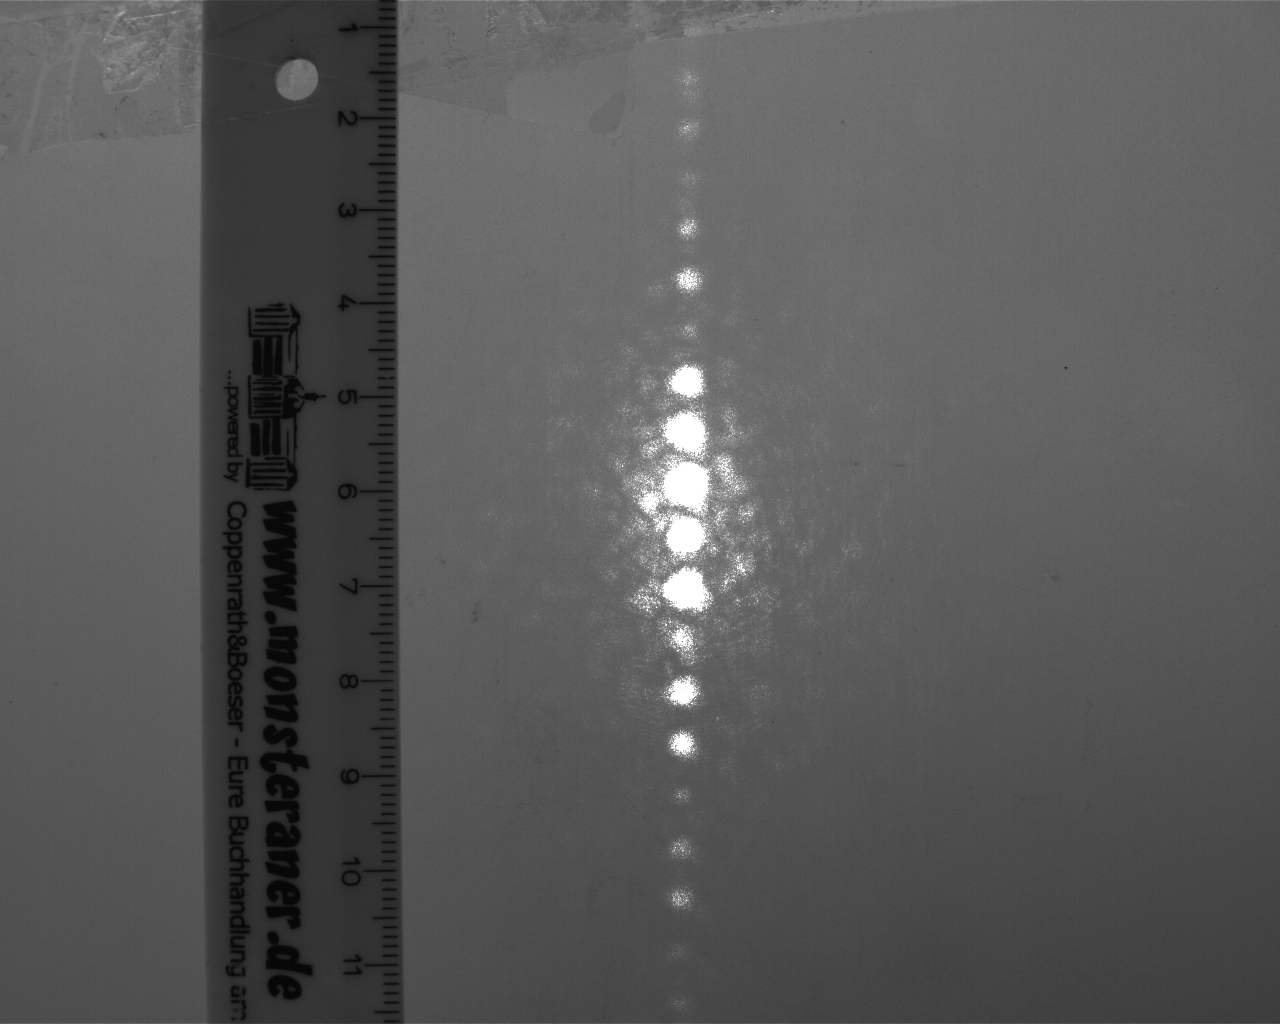
\includegraphics[width=\textwidth]{raw/1/1_fern_bild}
            \caption%
            {Kamera, $d=\SI{2580}{mm}$}
            \label{fig_1_fern_bild}
        \end{subfigure}
        \hfill
        \begin{subfigure}[b]{0.55\textwidth}
            \centering
            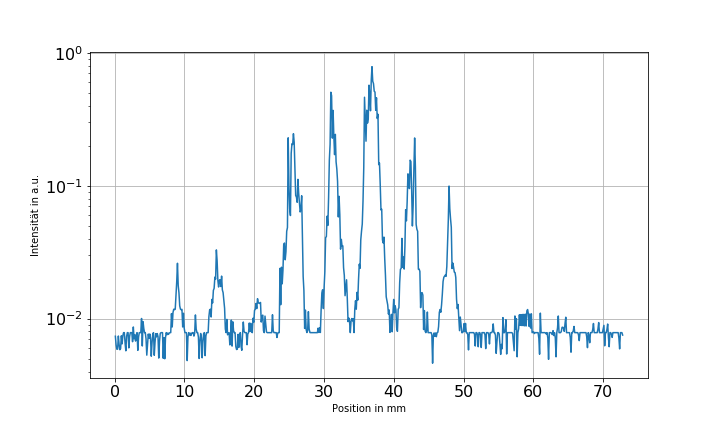
\includegraphics[width=\textwidth]{img/1/1_fern_plot}
            \caption[]%
            {Profil, $d=\SI{2580}{mm}$}
            \label{fig_1_fern_plot}
        \end{subfigure}
        \vskip\baselineskip
        \begin{subfigure}[b]{0.4\textwidth}
            \centering
            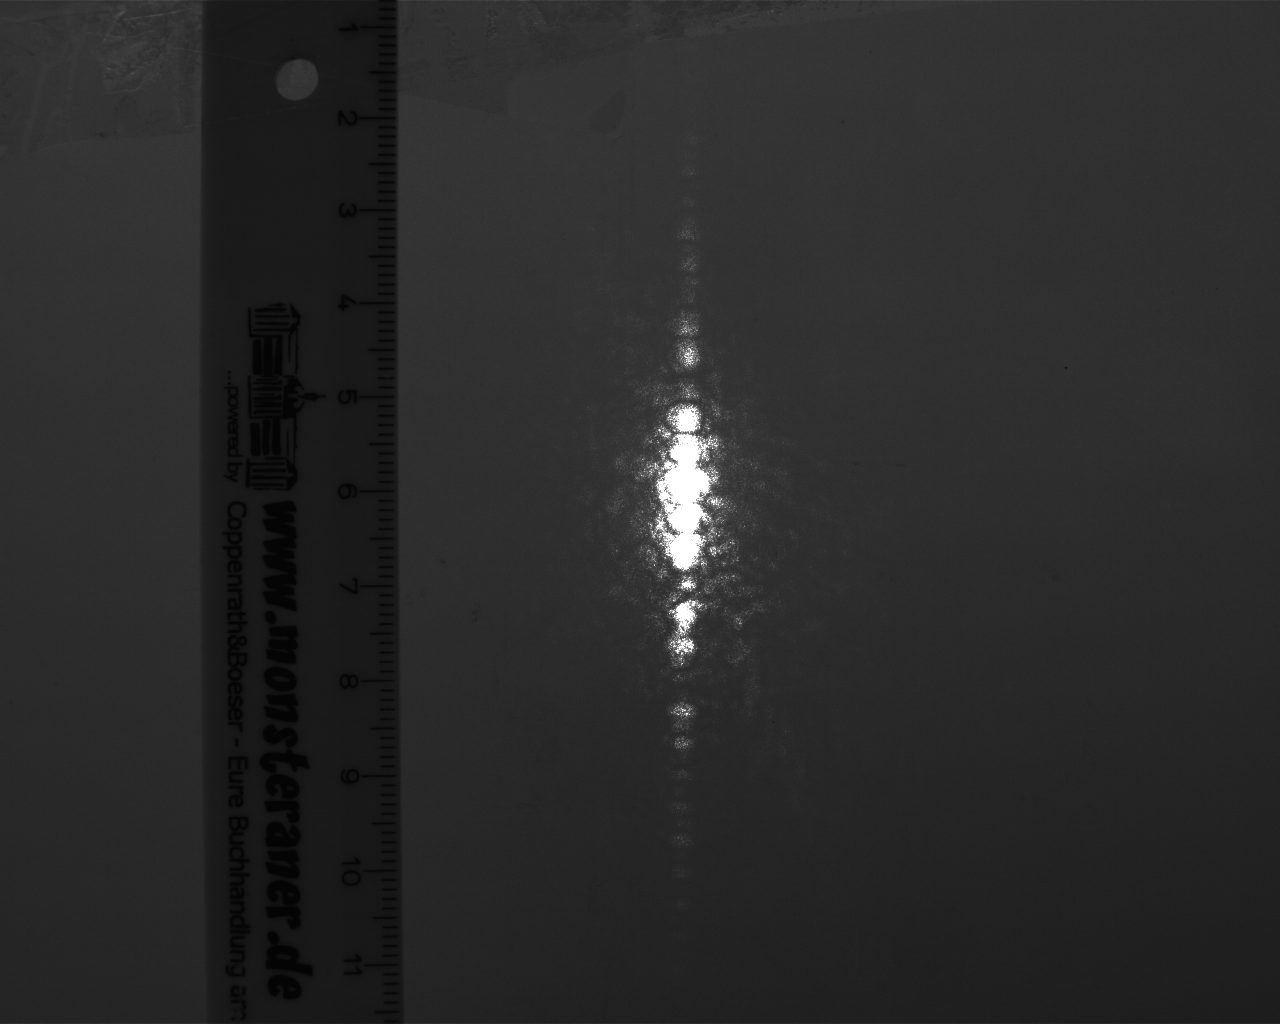
\includegraphics[width=\textwidth]{raw/1/1_mittel_bild}
            \caption[]%
            {Kamera, $d=\SI{1620}{mm}$}
            \label{fig_mittel_bild}
        \end{subfigure}
        \quad
        \begin{subfigure}[b]{0.55\textwidth}
            \centering
            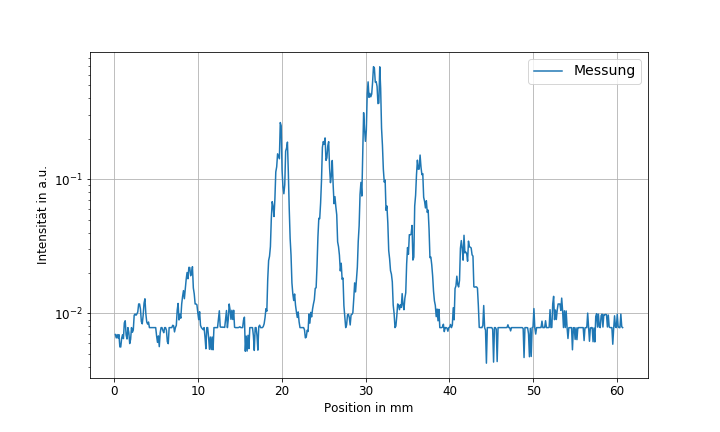
\includegraphics[width=\textwidth]{img/1/1_mittel_plot}
            \caption[]%
            {Profil, $d=\SI{1620}{m}$}
            \label{fig_mittel_plot}
        \end{subfigure}
        \vskip\baselineskip
        \begin{subfigure}[b]{0.4\textwidth}
            \centering
            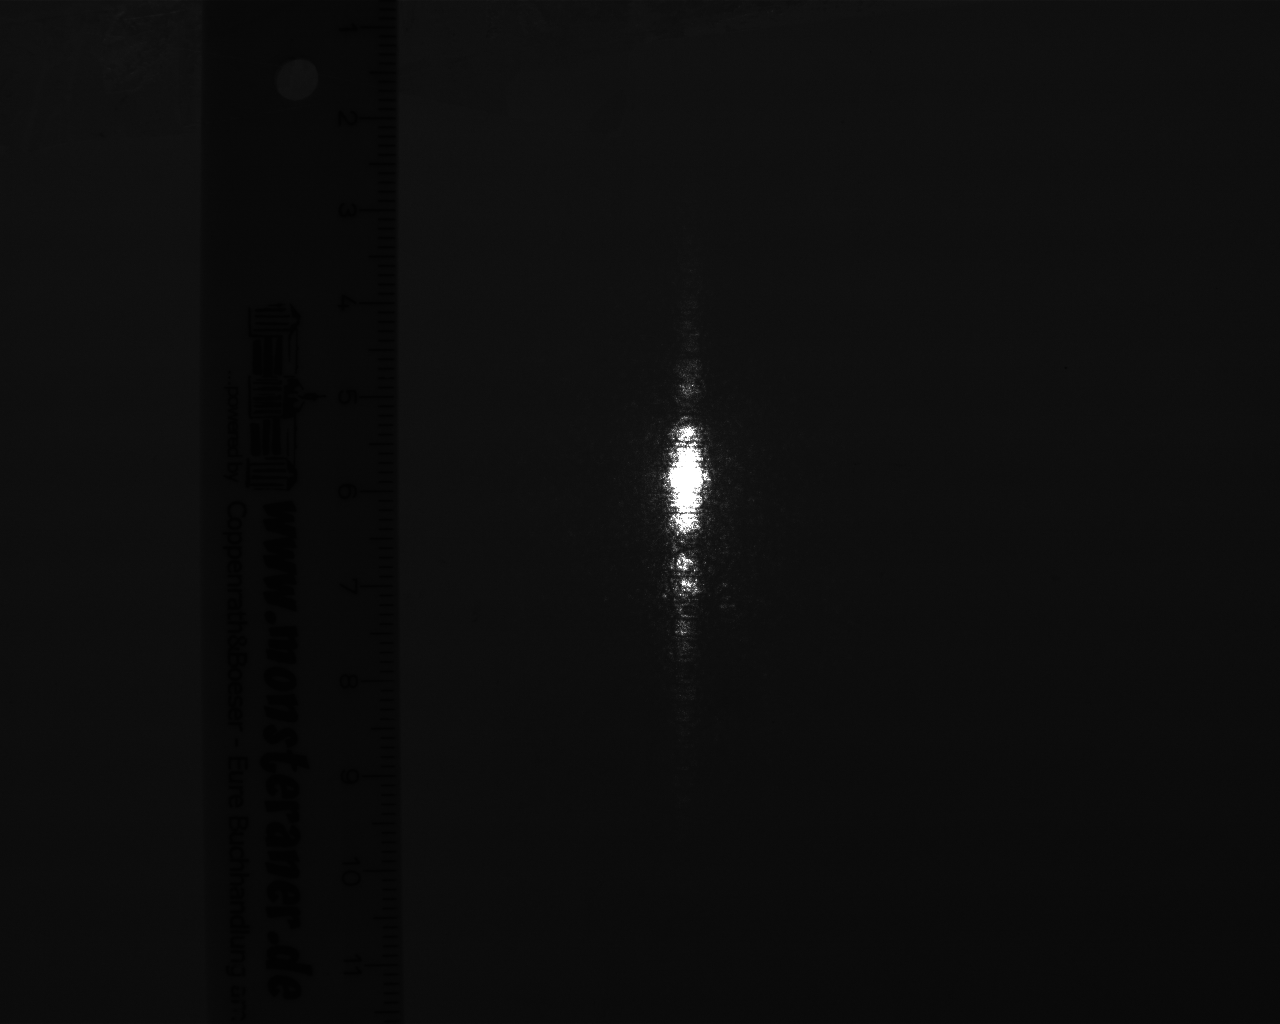
\includegraphics[width=\textwidth]{raw/1/1_mittel2_bild}
            \caption[]%
            {Kamera, $d=\SI{1060}{mm}$}
            \label{fig_mittel2_bild}
        \end{subfigure}
        \quad
        \begin{subfigure}[b]{0.55\textwidth}
            \centering
            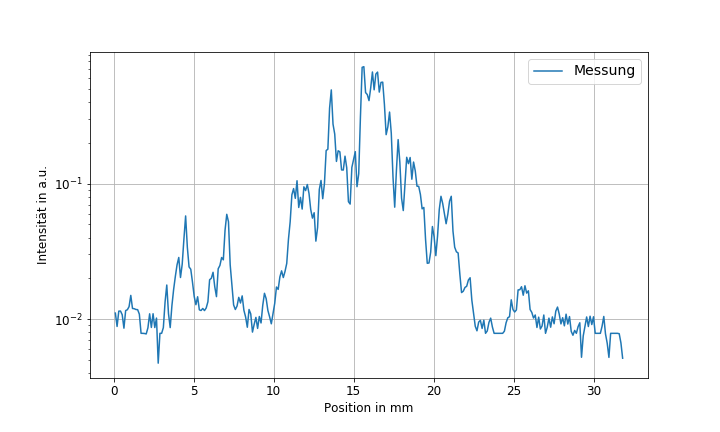
\includegraphics[width=\textwidth]{img/1/1_mittel2_plot}
            \caption[]%
            {Profil, $d=\SI{1060}{m}$}
            \label{fig_mittel2_plot}
        \end{subfigure}
        \caption%
        {
				Kameraaufnahmen und Intensitätsprofile für verschiedene Abstände $d$.
				Die Profile wurden aus anderen Bildern, mit geringerer Belichtungszeit extrahiert.
				Die x-Achse \enquote{Position} sagt nichts über die absolute Position des Maximums aus, sondern dient lediglich dem Bestimmen von Abständen zwischen Peaks.
				}
        \label{fig_1_mix_1}
    \end{figure}
	\begin{figure}[H]\ContinuedFloat
        \centering
        \begin{subfigure}[b]{0.4\textwidth}
            \centering
            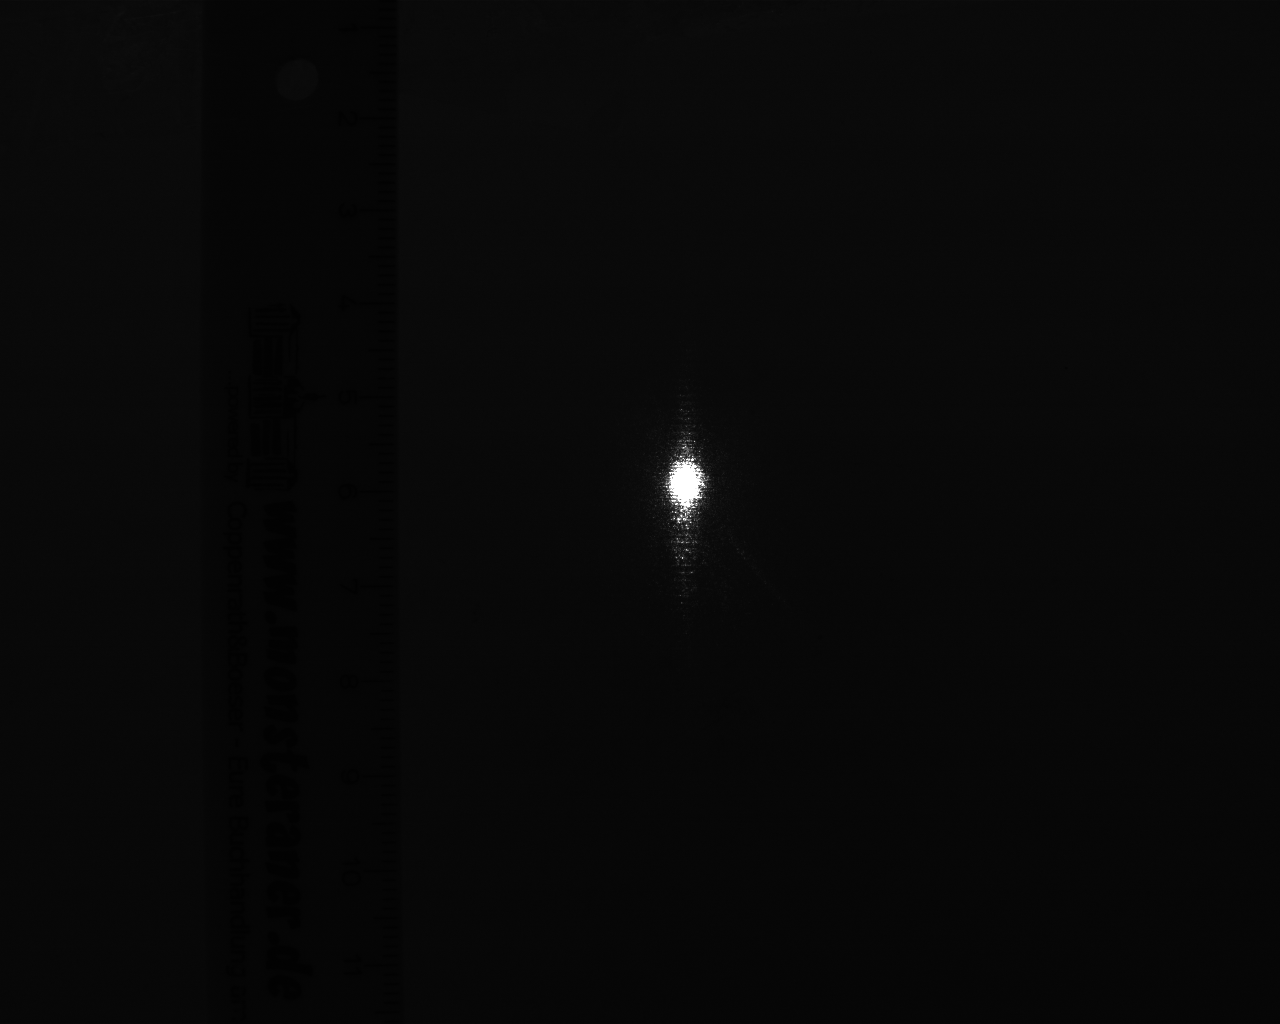
\includegraphics[width=\textwidth]{raw/1/1_nah_bild}
            \caption%
            {Kamera, $d=\SI{370}{mm}$}
            \label{fig_1_nah_bild}
        \end{subfigure}
        \hfill
        \begin{subfigure}[b]{0.55\textwidth}
            \centering
            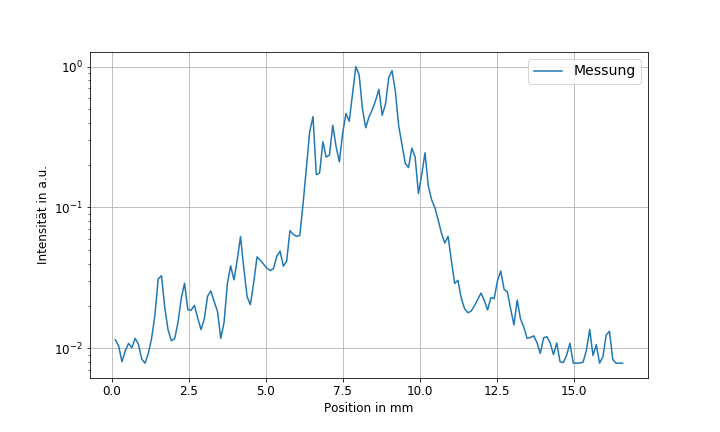
\includegraphics[width=\textwidth]{img/1/1_nah_plot}
            \caption[]%
            {Profil, $d=\SI{370}{mm}$}
            \label{fig_1_nah_plot}
        \end{subfigure}
        \vskip\baselineskip
        \begin{subfigure}[b]{0.4\textwidth}
            \centering
            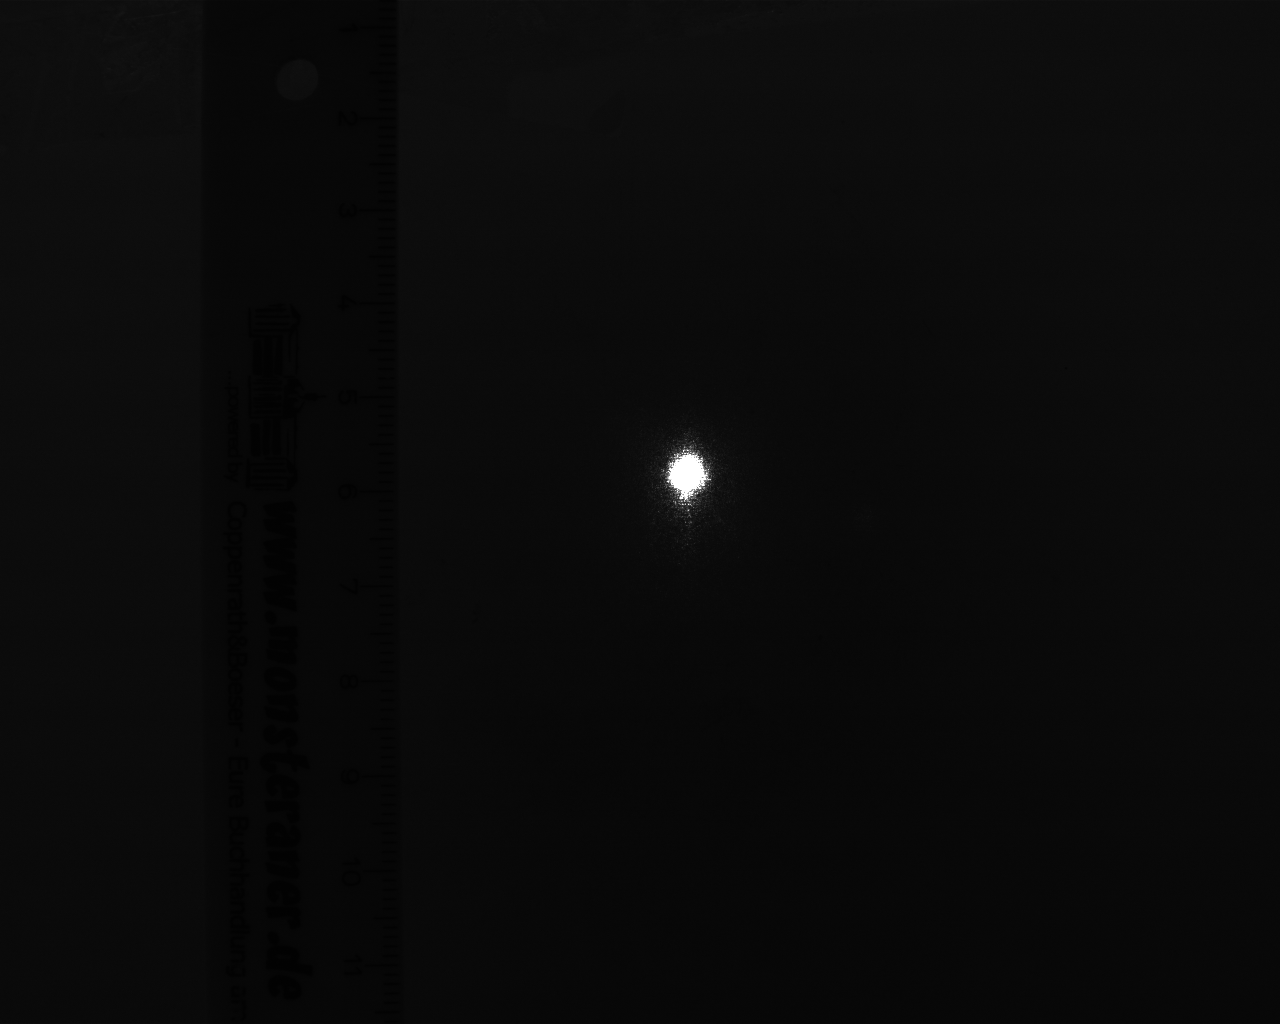
\includegraphics[width=\textwidth]{raw/1/1_ultra_bild}
            \caption[]%
            {Kamera, $d=\SI{150}{mm}$}
            \label{fig_ultra_bild}
        \end{subfigure}
        \quad
        \begin{subfigure}[b]{0.55\textwidth}
            \centering
            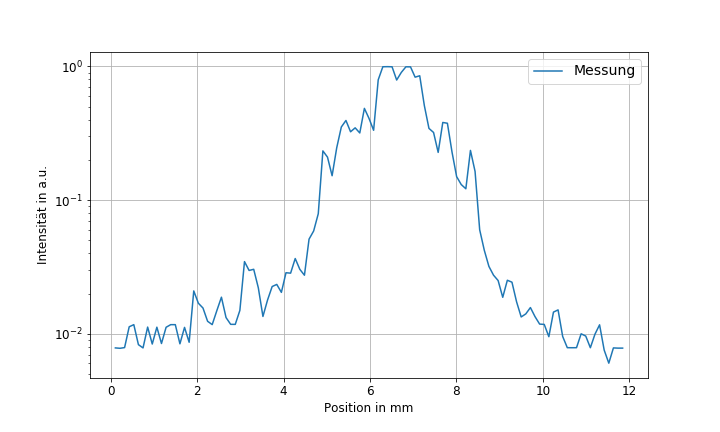
\includegraphics[width=\textwidth]{img/1/1_ultra_plot}
            \caption[]%
            {Profil, $d=\SI{150}{m}$}
            \label{fig_ultra_plot}
        \end{subfigure}
        \caption%
        {
				Kameraaufnahmen und Intensitätsprofile für verschiedene Abstände $d$.
				Die Profile wurden aus anderen Bildern, mit geringerer Belichtungszeit extrahiert.
				Die x-Achse \enquote{Position} sagt nichts über die absolute Position des Maximums aus, sondern dient lediglich dem Bestimmen von Abständen zwischen Peaks. (Forts.)
				}
        \label{fig_1_mix_2}
    \end{figure}
		%TODO wie zählt der die Unterpunkte weiter und wieso ist das beides dieselbe Nummer? Und macht man das so, dass man dann bei beiden die caption hinschreibt und Abbildung 4 stehen hat? Und wie mache ich das mit cref? der geht dann halt auf abb. 4 egal, welches label ich nehme.
	\subsubsection*{Diskussion}
	% Bezug/Nutzen oder sonst was
	% auch hier die Hypothese wiederholen
	% keine Messwerte hier, nach manchen Menschen, zumindest "direkt" erstellte Diagramme net hier, auch wenn Lesbarkeit-bla
	In \cref{fig_1_mix_1} kann man deutlich erkennen, dass für einen großen Abstand zwischen Gitter und Schirm das erwartete Beugungsbild bis zu hohen Beugungsordnungen zu erkennen ist.
	Je geringer der Abstand jedoch wird, desto schlechter sind die einzelnen Ordnungen zu unterscheiden, da hier die Fresnel-Beugung bzw. der Übergang zwischen Fresnel- und Fraunhofer-Beugung sichtbar wird.
	Dies entspricht den Erwartungen, da gemäß der Fraunhofer-Beugung (vgl. \cref{sec_fraunhofer}) erst im Fernfeld das Beugungsbild in der in \cref{sec_gitterbeug} auftritt.

	\subsection{Bestimmung der Gitterkonstanten}

	\subsubsection*{Methode}

	Es wird derselbe Aufbau wie zuvor verwendet (vgl. \cref{fig_nahfern}).
	Dann wird mit einem Abstand von \SI{2,715}{m} zwischen Gitter und Schirm das Beugungsbild für fünf verschiedene Gitter aufgenommen.

	\subsubsection*{Beobachtung und Datenanalyse}
	% Allgemeine Beobachtungen
	% Einflüsse von veränderten Parametern auf Messung
 In \cref{fig_2_mix_1} sind die Intensitätsprofile mit Fits zum Bestimmen der Gitterkonstante von fünf Gittern aufgeführt.
 Diese wird ermittelt durch Auftragen der Position der Peaks gegen die Peakordnung.
 In den Grafiken sind in rot die Positionen der Peaks markiert, deren Position ist nicht immer eindeutig, unter anderem wegen der Überbelichtung, welche jedoch nötig ist um höhere Peaks sichtbar zu machen, und die Unsicherheit wird mit \SI{1}{mm} abgeschätzt.
 In lila sind extrapolierte erwartete Peakpositionen markiert.

 Gemäß \cref{eq_beug} ist für kleine Winkel bzw. $k$:
 \begin{equation}
	 \label{eq_beug_verschieb}
	 u(k) = \frac{k\lambda d}{b} + \text{Verschiebung}
 \end{equation}
 Die Verschiebung ist Null wenn man Abstände von dem nullten Maximum misst und kann hier vernachlässigt werden, da die Information über die Gitterkonstante $b$ in der Steigung von der Geraden $u(k)$.

 Nun kann man nach \cref{eq_beug_verschieb} mit Abstand $d=\SI{2.715}{m}$ und Wellenlänge $\lambda=\SI{632.8}{nm}$ die Steigung $a$ in die Gitterkonstante $b=\lambda d/a$ umrechnen.
 Die Ergebnisse für die jeweiligen Gitter sind in \cref{tb_2_beug} aufgelistet.

\begin{figure}[H]
        \centering
        \begin{subfigure}[b]{0.475\textwidth}
            \centering
            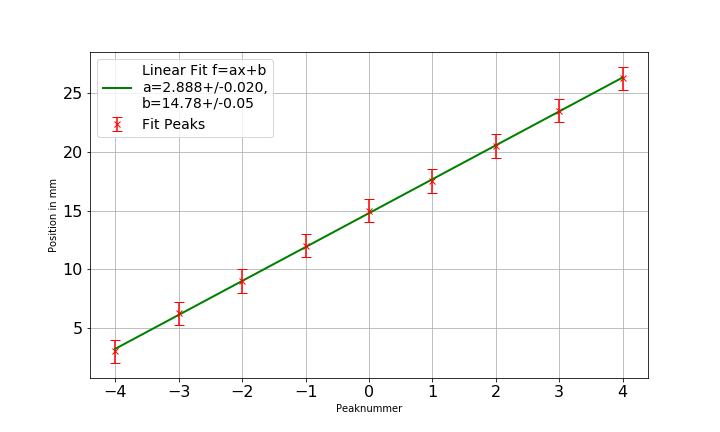
\includegraphics[width=\textwidth]{img/2/2_gitter_g1}
            \caption%
            {Profil, Gitter 1}
            \label{fig_2_profil_g1}
        \end{subfigure}
        \hfill
        \begin{subfigure}[b]{0.475\textwidth}
            \centering
            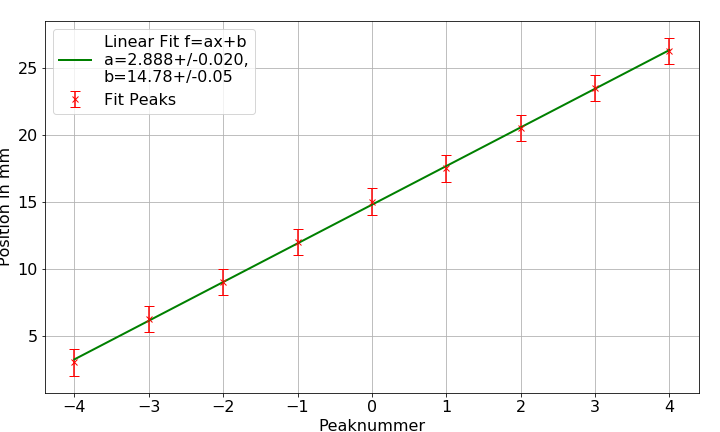
\includegraphics[width=\textwidth]{img/2/2_gitter_g1_fit}
            \caption[]%
            {Fit, Gitter 1}
            \label{fig_2_fit_g1}
        \end{subfigure}
        \begin{subfigure}[b]{0.475\textwidth}
            \centering
            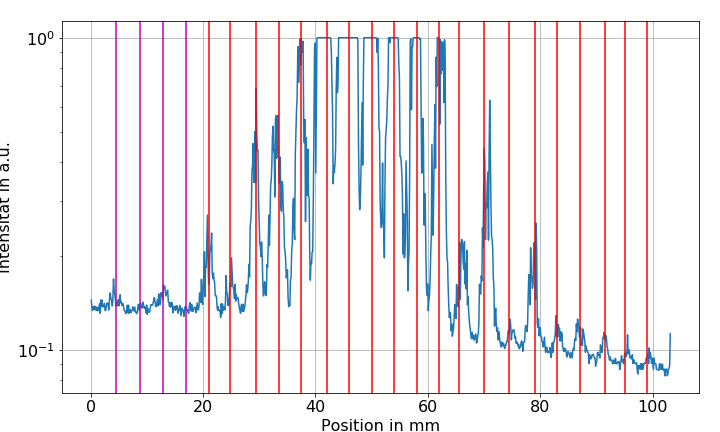
\includegraphics[width=\textwidth]{img/2/2_gitter_g2}
            \caption%
            {Profil, Gitter 2}
            \label{fig_2_profil_g2}
        \end{subfigure}
        \hfill
        \begin{subfigure}[b]{0.475\textwidth}
            \centering
            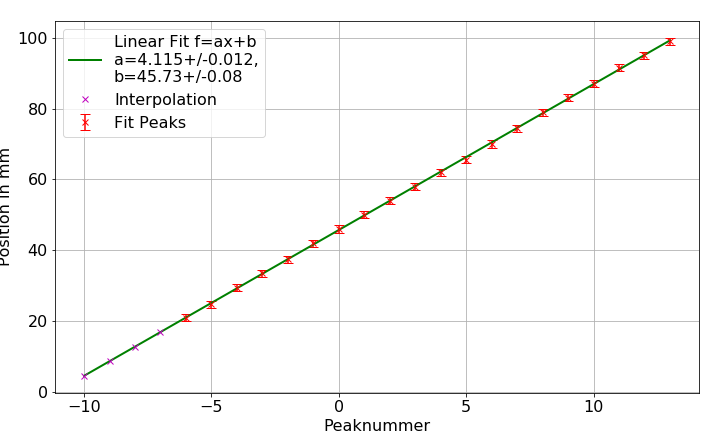
\includegraphics[width=\textwidth]{img/2/2_gitter_g2_fit}
            \caption[]%
            {Fit, Gitter 2}
            \label{fig_2_fit_g2}
        \end{subfigure}
        \begin{subfigure}[b]{0.475\textwidth}
            \centering
            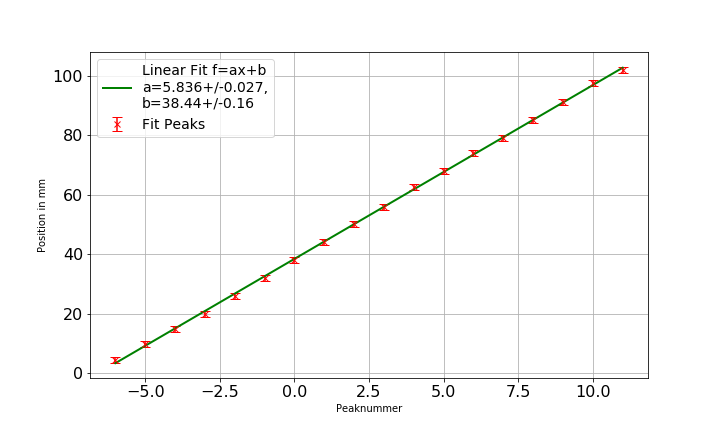
\includegraphics[width=\textwidth]{img/2/2_gitter_g3}
            \caption%
            {Profil, Gitter 3}
            \label{fig_2_profil_g3}
        \end{subfigure}
        \hfill
        \begin{subfigure}[b]{0.475\textwidth}
            \centering
            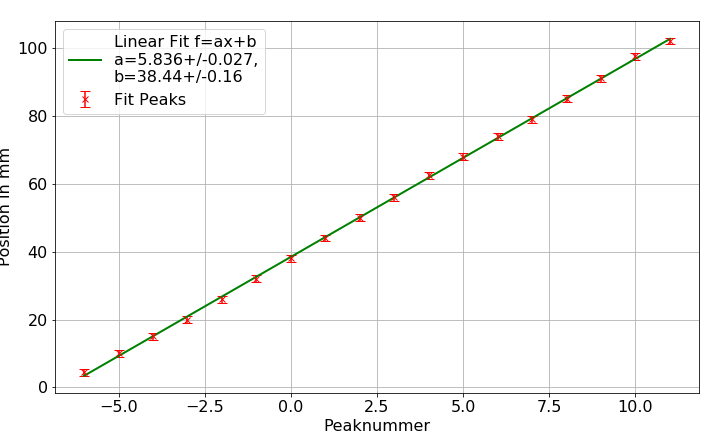
\includegraphics[width=\textwidth]{img/2/2_gitter_g3_fit}
            \caption[]%
            {Fit, Gitter 3}
            \label{fig_2_fit_g3}
        \end{subfigure}
        \caption%
        {
				Intensitätsprofile und Peakfits für verschiedene Gitter.
				Die x-Achse \enquote{Position} sagt nichts über die absolute Position des Maximums aus, sondern dient lediglich dem Bestimmen von Abständen zwischen Peaks.
				}
        \label{fig_2_mix_1}
    \end{figure}
	\begin{figure}[H]\ContinuedFloat
        \centering

				\begin{subfigure}[b]{0.475\textwidth}
            \centering
            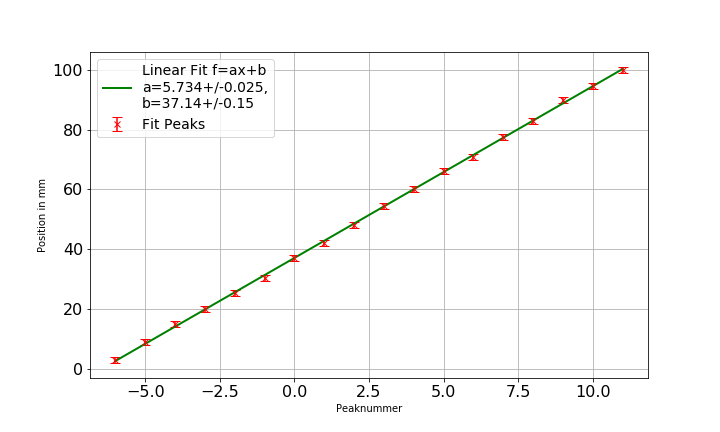
\includegraphics[width=\textwidth]{img/2/2_gitter_g4}
            \caption%
            {Profil, Gitter 4}
            \label{fig_2_profil_g4}
        \end{subfigure}
        \hfill
        \begin{subfigure}[b]{0.475\textwidth}
            \centering
            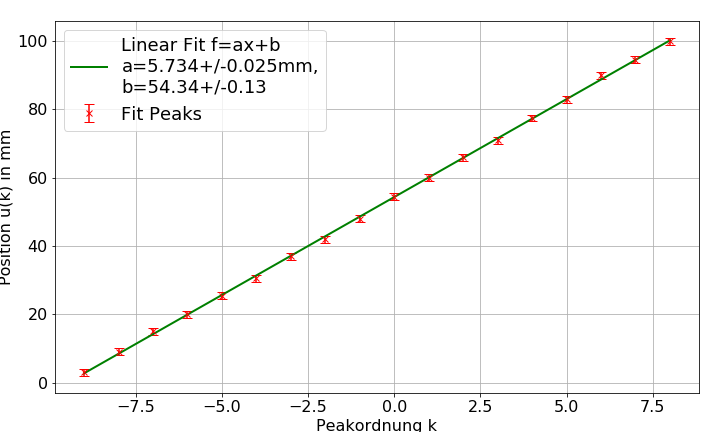
\includegraphics[width=\textwidth]{img/2/2_gitter_g4_fit}
            \caption[]%
            {Fit, Gitter 4}
            \label{fig_2_fit_g4}
        \end{subfigure}
        \begin{subfigure}[b]{0.475\textwidth}
            \centering
            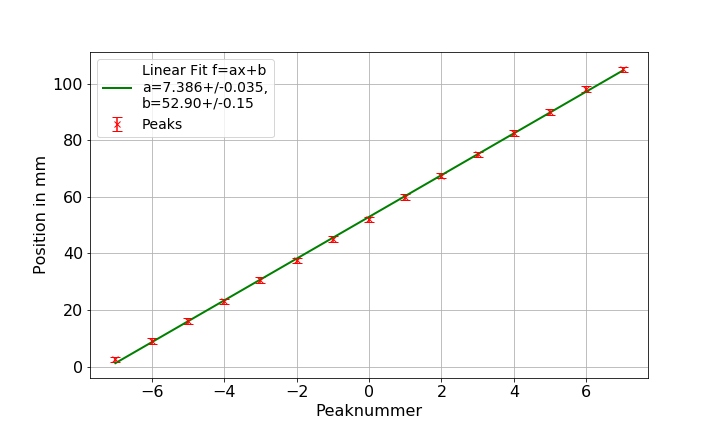
\includegraphics[width=\textwidth]{img/2/2_gitter_g5}
            \caption%
            {Profil, Gitter 5}
            \label{fig_2_profil_g5}
        \end{subfigure}
        \hfill
        \begin{subfigure}[b]{0.475\textwidth}
            \centering
            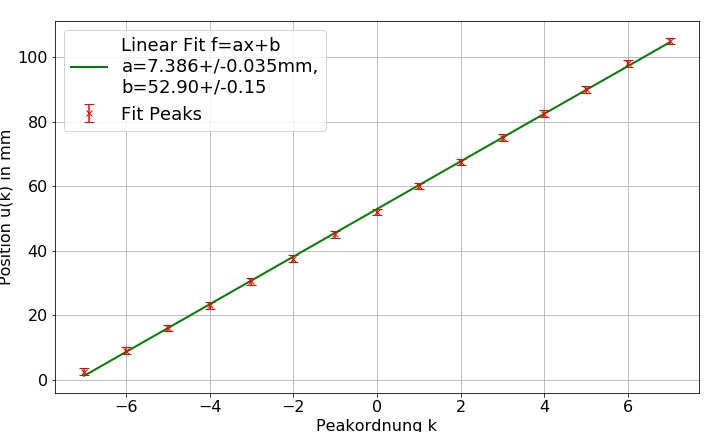
\includegraphics[width=\textwidth]{img/2/2_gitter_g5_fit}
            \caption[]%
            {Fit, Gitter 5}
            \label{fig_2_fit_g5}
        \end{subfigure}
        \caption%
        {
				Intensitätsprofile und Peakfits für verschiedene Gitter.
				Die x-Achse \enquote{Position} sagt nichts über die absolute Position des Maximums aus, sondern dient lediglich dem Bestimmen von Abständen zwischen Peaks. (Forts.)
				}
        \label{fig_2_mix_2}
    \end{figure}

\begin{table}[H]
		\centering
		\begin{tabular}{ c | c | c }
			 Gitternummer & Steigung $a$ in \si{mm} & Gitterkonstante $b$ in \si{mm} \\ \hline
			 \input{res/tb_2_beug}
		\end{tabular}
		\caption{
		Aus der Steigung $a$ mit \cref{eq_beug} berechnete Gitterkonstanten $b$.
		}
		\label{tb_2_beug}
\end{table}
	\subsubsection*{Diskussion}
	% Bezug/Nutzen oder sonst was
	% auch hier die Hypothese wiederholen
	% keine Messwerte hier, nach manchen Menschen, zumindest "direkt" erstellte Diagramme net hier, auch wenn Lesbarkeit-bla

	\subsection{Fouriertransformation mit einer Linse}

	\subsubsection*{Methode}

		Der vorherige Versuchsteil wird mit dem Unterschied, dass sich nun eine Linse zwischen Schirm und Gitter befindet, widerholt.
		Die Linse wird so eingebaut, dass sich Schirm und Gitter in je einer der Fokusebenen befinden.

	\begin{figure}[H]
			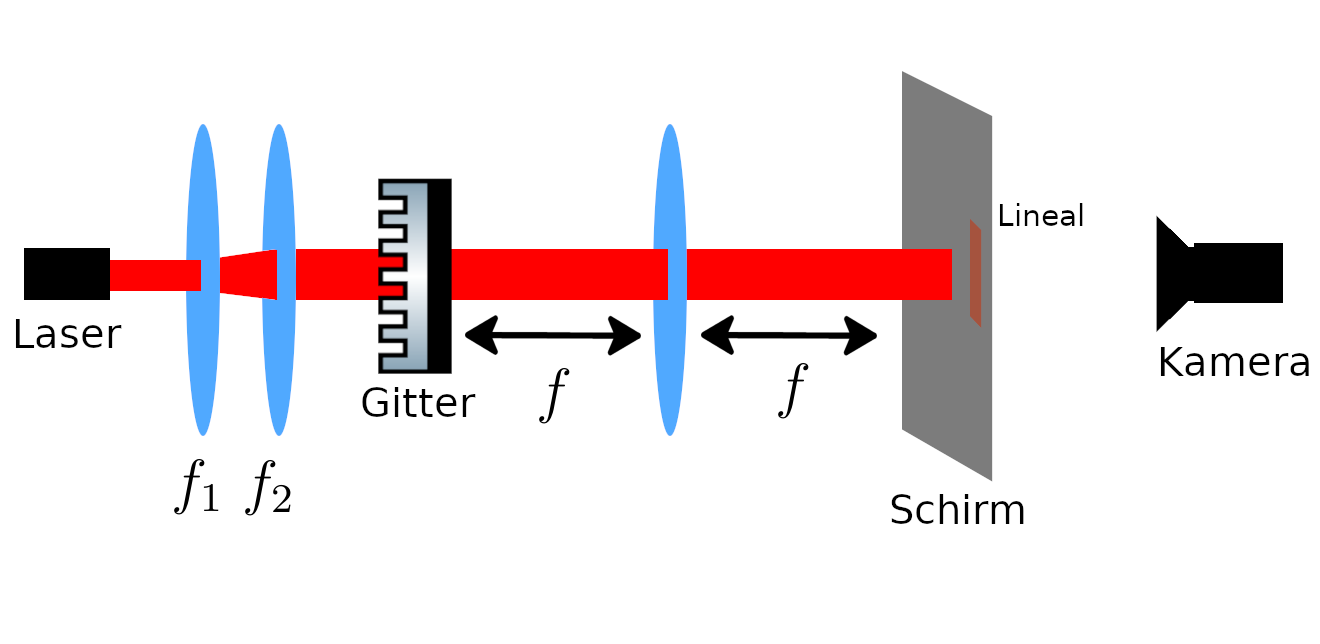
\includegraphics[width=1\linewidth]{img/gitterlinse}
			\caption{
				Aufbau zur Bestimmung der Abstände der Beugungsordnungen. Die zusätzlich eingebaute Linse steht im Abstand $f=\SI{500}{mm}$ zu Gitter und Schirm.
			}
			\label{fig_gitterlinse}
	\end{figure}

	\subsubsection*{Beobachtung und Datenanalyse}
	% Allgemeine Beobachtungen
	% Einflüsse von veränderten Parametern auf Messung
	%TODO Überstrahlung nahe 0. Ordnung verhindert Zählen -> Extrapolation der Ordnung aus Abstand
	%TODO bei g1 nichts zu erkennen -> Alternativversuche -> immer noch nicht.

	\subsubsection*{Diskussion}
	% Bezug/Nutzen oder sonst was
	% auch hier die Hypothese wiederholen
	% keine Messwerte hier, nach manchen Menschen, zumindest "direkt" erstellte Diagramme net hier, auch wenn Lesbarkeit-bla
%TODO man verlässt sich halt nicht auf Fernfeld, sondern bringt das Bild in die Endlichkeit.

Durch die Verwendung einer Linse wird die Fouriertransformation im Nahfeld dargestellt. %TODO so hat es Merkel formuliert.
Deswegen überrascht nicht, dass hier auch bei einem geringen Abstand vom Schirm das Beugungsbild zu erkennen ist.
Der Schirm muss natürlich im Fokus der Linse stehen, damit das Bild scharf ist.


	\subsection{Fourierfilterung}

	\subsubsection*{Methode}

		Der Strahl wird mit einem Linsenpaar auf einen Durchmesser von etwa \SI{50}{mm} aufgeweitet und kollimiert.
		Es wird ein 4-f-Aufbau zur Fourierfilterung verwendet.
		Dieser ist in \cref{fig_4f} dargestellt.
		Dann werden mehrere Messungen mit unterschiedlichen Objekten und Filtern durchgeführt.

	\begin{figure}[H]
			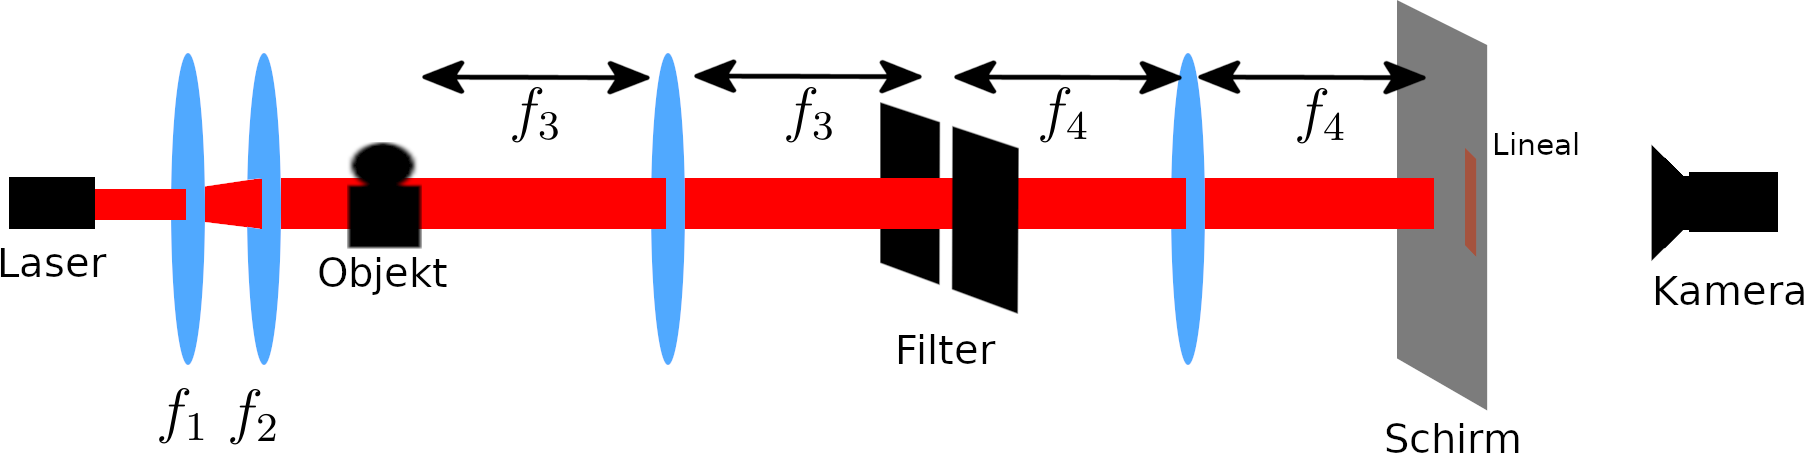
\includegraphics[width=1\linewidth]{img/4f}
			\caption{
				4-f-Aufbau zur Fourierfilterung. $f_1= \SI{5}{mm}$, $f_2 = f_3 = f_4 = \SI{500}{mm}$. Es werden verschiedene Objekte und Filter verwendet.
			}
			\label{fig_4f}
	\end{figure}


		Zunächst wird der Schriftzug \enquote{Fourier} überlagert mit einem senkrechten Gitter als Objekt verwendet.
		Durch einen Tiefpassfilter wird dieser aus dem Bild entfernt.
		Der Tiefpassfilter wird durch einen schmalen horizontalen Spalt realisiert.

		Dann wird ein Bruch als Objekt verwendet, bei dem der Nenner mit einem Gitter überlagert ist.
		Um den Zähler aus dem Bruch zu entfernen, wird ein eindimensionaler Hochpassfilter in Form einer Nadel verwendet.
		%TODO Hier haben wir, denke ich, verkackt. Wir haben den Nenner entfernt.

		Nun wird ein Quadratgitter und ein Spalt als eindimensionaler Tiefpassfilter verwendet.
		Der Spalt wird im Winkel von \SI{0}{\degree}, \SI{45}{\degree} und \SI{90}{\degree} eingesetzt.

		Es wird als Objekt eine Schraube und als Filter ein Hochpassfilter in Form eines Kreises auf einer durchsichtigen Folie verwendet.

		Zuletzt wird, um die Dunkelfeldmethode zu verwenden, wie zuvor ein Hochpassfilter eingesetzt.
		Als Objekt werden die aufsteigenden Luftströme über einer Kerzenflamme verwendet.
		Damit diese besser sichtbar werden, werden Luftverwirbelungen per Hand eingebracht.

	\subsubsection*{Beobachtung und Datenanalyse}
	% Allgemeine Beobachtungen
	% Einflüsse von veränderten Parametern auf Messung

	\subsubsection*{Diskussion}
	% Bezug/Nutzen oder sonst was
	% auch hier die Hypothese wiederholen
	% keine Messwerte hier, nach manchen Menschen, zumindest "direkt" erstellte Diagramme net hier, auch wenn Lesbarkeit-bla
%TODO fourierschriftzug: Buchstabenfrequenz kleiner als gitter. Je mehr wegefiltert, desto unschärfer der Schriftzug.

	\section{Schlussfolgerung}
	% Rückgriff auf Hypothese und drittes Nennen dieser

	% Quellen zitieren, Websiten mit Zugriffsdatum
	% Verweise auf das Laborbuch (sind erlaubt)
	% Tabelle + Bilder mit Beschriftung
	\printbibliography
\end{document}


%TODO Einheiten bisschen anpassen, also alle Brennweiten in Millimeter und alle Abstände gleichmäßig.
